%%%%%%%%%%%%%%%%%%%%%%%%%%%%%%%%%%%%%%%%%%%%%%%%%%%%%
% Rapport S2 - TER PICOPATT
%%%%%%%%%%%%%%%%%%%%%%%%%%%%%%%%%%%%%%%%%%%%%%%%%%%%%
\documentclass{article}

\usepackage[T1]{fontenc}
\usepackage[utf8]{inputenc}
\usepackage[french]{babel}
\usepackage{lmodern}
\usepackage[margin=1in]{geometry}
\usepackage{setspace}
\onehalfspacing
\setlength{\parindent}{0pt}
\setlength{\parskip}{0.45em}
\emergencystretch=2em

\usepackage{graphicx}
\graphicspath{{./}{../../}}
\usepackage{float}
\usepackage{caption}
\usepackage{subcaption}
\captionsetup{font=small,labelfont=bf}
\usepackage{booktabs}
\usepackage{tabularx}
\usepackage{array}
\usepackage{csquotes}
\usepackage{hyperref}
\hypersetup{pdfborder={0 0 0}}
\usepackage[
  backend=biber,
  style=numeric,
  sorting=none
]{biblatex}
\addbibresource{rapport/s2/references.bib}
\usepackage{titlesec}
\renewcommand{\thesection}{\arabic{section}.}
\renewcommand{\thesubsection}{\arabic{section}.\arabic{subsection}.}
\renewcommand{\thesubsubsection}{\arabic{section}.\arabic{subsection}.\arabic{subsubsection}.}
\titleformat{\section}{\normalfont\Large\bfseries}{\thesection}{0.8em}{}
\newcolumntype{Y}{>{\raggedright\arraybackslash}X}

\newcommand{\webappscreen}[2]{%
  \IfFileExists{#1}{%
    \includegraphics[width=\textwidth]{#1}%
  }{%
    \fbox{%
      \begin{minipage}[c][0.26\textwidth][c]{0.92\textwidth}
        \centering
        \small Capture à insérer : #2\\[0.15cm]
        \footnotesize\texttt{\detokenize{#1}}
      \end{minipage}%
    }%
  }%
}

\begin{document}

\hypersetup{pageanchor=false}
\begin{titlepage}
  \centering
  \vspace*{0.3cm}
  {\Large TER - Projet ANR PICOPATT\\[0.5cm]}
  \rule{\textwidth}{0.9pt}\\[0.5cm]
  {\Large \textbf{Prédiction et spatialisation de la température moyenne radiante à Montpellier}}\\[0.35cm]
  {\large Rapport d'avancement TER du 21 mai 2026}\\[0.2cm]
  \rule{\textwidth}{0.9pt}\\[0.65cm]

  \large
  Réalisé par\\[0.1cm]
  Ayoub AKKOUH,\\
  Anthony COMBES-AGUÉRA,\\
  Youssef EL ALAOUI,\\
  et Dylla Liesse IZERE\\[0.25cm]

  \rule{0.5\textwidth}{0.9pt}\\[0.25cm]

  Encadré par\\[0.1cm]
  Sandra BRINGAY,\\
  Luc Étienne POMMÉ-CASSIÉROU,\\
  Vincent RAVENEAU,\\
  et Maximillien SERVAJEAN\\[0.8cm]

  \begin{minipage}[c]{0.3\textwidth}
    \centering
    
\includegraphics[width=0.8\textwidth]{rapport/s2/Images/Logo/logo-lirmm.jpg}
  \end{minipage}
  \hfill
  \begin{minipage}[c]{0.3\textwidth}
    \centering
    
\includegraphics[width=0.95\textwidth]{rapport/s2/Images/Logo/logo picopatt.png}
  \end{minipage}
  \hfill
  \begin{minipage}[c]{0.3\textwidth}
    \centering
    
\includegraphics[width=0.8\textwidth]{rapport/s2/Images/Logo/logo-upvm_4.jpg}
  \end{minipage}

  \vfill
  \footnotesize
  Année universitaire 2025-2026
\end{titlepage}

\newpage
\thispagestyle{empty}
\vspace*{3cm}
\begin{center}
{\Large \textbf{Remerciements}}
\end{center}

\vspace{1cm}
Nous tenons à remercier nos encadrants, Sandra Bringay, Luc Étienne Pommé-Cassiérou, Vincent Raveneau et Maximillien Servajean, pour leur suivi tout au long du semestre. Leurs retours nous ont permis de mieux structurer le travail, de préciser les objectifs de modélisation et de prendre plus de recul sur l'évaluation des résultats.

Nous remercions également les personnes impliquées dans le projet PICOPATT pour les données, les outils et le contexte scientifique mis à disposition. Ces éléments ont été indispensables pour passer de l'analyse exploratoire menée au S1 à une démarche de prédiction et de spatialisation au S2.

\newpage
\hypersetup{pageanchor=true}
\setcounter{page}{1}
\tableofcontents
\newpage

%%%%%%%%%%%%%%%%%%%%%%%%%%%%%%%%%%%%%%%%%%%%%%%%%%%%%
\section{Introduction et contexte du TER}
%%%%%%%%%%%%%%%%%%%%%%%%%%%%%%%%%%%%%%%%%%%%%%%%%%%%%

\subsection{Missions initiales du TER}

Le TER s'inscrit dans le projet PICOPATT, qui étudie les picoclimats urbains à partir de mesures mobiles réalisées dans la ville \cite{picopatt-site}. Dès le début du projet, la mission principale était de partir des séries temporelles produites par le chariot pour mieux identifier et caractériser ces situations climatiques très locales. Les données ne devaient donc pas être seulement décrites point par point. Elles devaient être transformées en profils plus lisibles, capables de résumer la dynamique d'un passage et de faire apparaître des formes récurrentes.
L'objectif initial reposait sur la construction de silhouettes picoclimatiques. Une silhouette correspond à un profil typique, obtenu à partir de mesures qui se ressemblent dans l'espace et dans le temps. Cette idée devait servir de base à des tâches plus avancées comme la comparaison de passages, la classification de contextes, la détection d'anomalies ou la prévision. Les premières étapes prévues concernaient donc le nettoyage des séries, la gestion des valeurs manquantes, la segmentation des parcours, le calcul de statistiques simples et la visualisation des profils. Dans un second temps, des modèles d'apprentissage de représentations pouvaient être envisagés pour apprendre automatiquement des profils compacts.

Cette mission a évolué au contact des données réellement disponibles. Les mesures PICOPATT sont riches, mais elles sont aussi très denses et fortement liées au parcours suivi. Le travail du S2 reprend donc la question de la représentation des profils, mais sous un angle plus opérationnel. Il cherche à savoir si certaines variables disponibles au-delà du seul chariot peuvent aider à prédire \texttt{tmrt}, puis à produire une carte dense de cette variable sur Montpellier.

\subsection{Continuité avec le rapport S1}

Le Semestre 1 s'arrêtait sur la compréhension des mesures. Il mettait en évidence des profils cohérents avec la morphologie des parcours et avec la dynamique journalière. Les variables radiatives, en particulier les composantes de rayonnement solaire, apparaissaient fortement liées à \texttt{tmrt}. Les analyses par \texttt{M\_slot} (passage à différentes heures pour un même parcours) montraient aussi que certains motifs reviennent aux mêmes zones du trajet, tandis que le niveau moyen change selon la date, l'heure et les conditions météorologiques.

Le Semestre 2 reprend à cet endroit. Il ne repart pas de zéro et ne remplace pas les analyses du S1. Il s'appuie sur elles pour passer d'une lecture exploratoire des profils à une question de modélisation. La difficulté devient alors plus précise : construire un modèle utile sans utiliser uniquement des variables que l'on ne peut mesurer qu'avec le chariot. Cette contrainte est centrale, car l'objectif n'est pas seulement de retrouver les points déjà parcourus, mais de préparer une prédiction plus dense dans l'espace.

Ce rapport suit donc volontairement l'ordre chronologique du semestre. Il commence par les données retenues et les raisons de ces choix. Il présente ensuite le premier modèle testé, les problèmes rencontrés pendant son évaluation, les solutions mises en place, puis la construction de la heatmap et de l'application web.

\subsection{Rappel du projet PICOPATT}

PICOPATT étudie les variations locales du climat urbain à une échelle très fine. Le projet s'intéresse aux différences que l'on peut observer entre une rue étroite, une place ouverte, un axe urbain plus large ou un espace plus exposé au vent. Ces différences peuvent être importantes pour les piétons, car elles modifient l'exposition au soleil, la ventilation, l'humidité locale et le confort thermique ressenti.

À Montpellier, les mesures utilisées dans le projet proviennent d'une station météorologique mobile installée sur un chariot. Les parcours étudiés sont au nombre de trois : Écusson, Boulevards et Antigone. Ces trois parcours représentent des formes urbaines contrastées. L'Écusson correspond à un tissu plus ancien et plus encaissé, les Boulevards alternent des axes et des espaces plus ouverts, tandis qu'Antigone présente des espaces plus larges et plus réguliers. Cette diversité donne un cadre pertinent pour observer des contrastes picoclimatiques.

Les photographies de \hyperref[fig:photos_parcours]{la figure~\ref{fig:photos_parcours}} illustrent ces trois contextes urbains.

\begin{figure}[H]
\centering
\begin{subfigure}[b]{0.3\textwidth}
    \centering
    
\includegraphics[width=\textwidth]{rapport/s2/Images/Parcours/Place de la Comédie.png}
    \caption{La place de la Comédie}
    \vspace{-0.3cm}
    \caption*{\footnotesize Boulevards}
    \label{fig:boulevards}
\end{subfigure}
\hspace{0.03\textwidth}
\begin{subfigure}[b]{0.3\textwidth}
    \centering
    
\includegraphics[width=\textwidth]{rapport/s2/Images/Parcours/3 Rue de la Verrerie Basse.png}
    \caption{La rue de la Verrerie Basse}
    \vspace{-0.3cm}
    \caption*{\footnotesize Écusson}
    \label{fig:ecusson}
\end{subfigure}
\hspace{0.03\textwidth}
\begin{subfigure}[b]{0.3\textwidth}
    \centering
    
\includegraphics[width=\textwidth]{rapport/s2/Images/Parcours/esplanade de l'europe.png}
    \caption{L'esplanade de l'Europe}
    \vspace{-0.3cm}
    \caption*{\footnotesize Antigone}
    \label{fig:antigone}
\end{subfigure}
\caption{Photographies représentatives des différents parcours de Montpellier.}
\vspace{-0.45cm}
\caption*{\footnotesize Source : Google Maps}
\label{fig:photos_parcours}
\end{figure}

Les tracés de \hyperref[fig:traces-parcours]{la figure~\ref{fig:traces-parcours}} montrent ensuite la forme des parcours suivis par le chariot.

\begin{figure}[H]
\centering    
\begin{subfigure}[b]{0.2\textwidth}
    \centering
    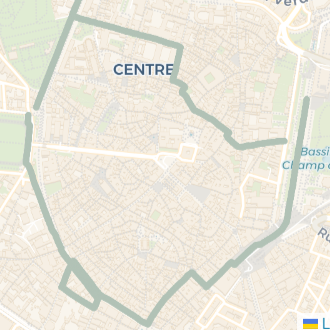
\includegraphics[width=\textwidth]{rapport/s1/Images/Parcours/boulevard.png}
    \caption{Boulevards}
    \label{fig:tracé_boulevard}
\end{subfigure}
\hspace{0.01\textwidth}
\begin{subfigure}[b]{0.2\textwidth}
    \centering
    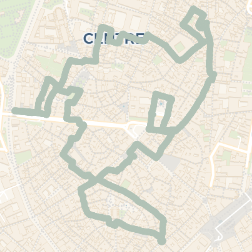
\includegraphics[width=\textwidth]{rapport/s1/Images/Parcours/ecusson.png}
    \caption{Écusson}
    \label{fig:tracé_ecusson}
\end{subfigure}
\hspace{0.01\textwidth}
\begin{subfigure}[b]{0.55\textwidth}
    \centering
    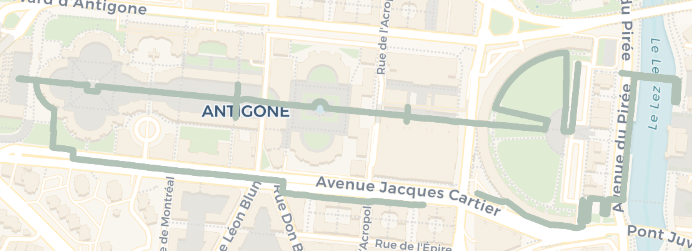
\includegraphics[width=\textwidth]{rapport/s1/Images/Parcours/antigone.png}
    \caption{Antigone}
    \label{fig:tracé_antigone}
\end{subfigure}
\caption{Captures d'écran des tracés des différents parcours.}
\vspace{-0.45cm}
\caption*{\footnotesize Source : Picopatt ExploreR (ADVANSE - LIRMM)}
\label{fig:traces-parcours}
\end{figure}

\subsection{État de l'art ciblé}

Les travaux sur les climats urbains montrent que les conditions thermiques locales dépendent fortement de la morphologie urbaine, de la couverture du sol, des matériaux et des usages. Les Local Climate Zones constituent un cadre classique pour décrire les grands contrastes entre tissus urbains \cite{stewart-oke-2012}. Ce cadre est utile pour comparer des quartiers ou des formes urbaines générales, mais PICOPATT se place à une échelle plus fine. Le projet observe la rue, la place, la façade, l'ombre portée et la position du piéton dans le parcours. À cette échelle, deux points proches peuvent déjà correspondre à des conditions radiatives différentes.

Cette différence d'échelle explique l'intérêt des mesures mobiles. Une station fixe décrit bien un point, mais elle ne suffit pas à suivre les variations rencontrées par un piéton en mouvement. Le chariot PICOPATT permet au contraire d'enregistrer des profils continus le long de parcours répétés. Cette approche est adaptée à l'étude des picoclimats, car elle conserve la forme du signal et les ruptures locales. Elle pose aussi une difficulté méthodologique importante. Les observations successives sont très proches dans le temps et dans l'espace, donc elles ne peuvent pas être traitées comme des points indépendants.

La variable \texttt{tmrt} occupe une place centrale dans l'analyse du confort thermique extérieur. Elle synthétise l'effet radiatif de l'environnement sur un individu et intervient dans des indices de confort comme \texttt{PET}. Son estimation reste délicate, car les méthodes fondées sur les mesures radiatives complètes, les globes noirs ou les modèles radiatifs ne sont pas équivalentes \cite{kruger-2014-tmrt}. Pour ce projet, ce point est essentiel. \texttt{tmrt} réagit fortement à l'ombre, à l'exposition solaire et aux surfaces urbaines proches. Elle est donc pertinente pour caractériser les contrastes locaux, mais elle est plus difficile à prédire qu'une variable atmosphérique plus lisse comme la température de l'air.

Le passage vers la modélisation impose aussi de distinguer les variables que l'on peut mesurer seulement sur les parcours et celles que l'on peut utiliser ailleurs. Les flux radiatifs embarqués décrivent très bien les points parcourus, mais ils ne sont pas disponibles sur toute la ville. Les variables météorologiques horaires donnent un contexte atmosphérique plus général, tandis que les embeddings géospatiaux AlphaEarth fournissent une description spatiale issue de données d'observation de la Terre \cite{brown-2025-alphaearth}. Le jeu Satellite Embedding V1 disponible dans Google Earth Engine rend ces représentations exploitables sur des points géographiques réguliers \cite{google-earth-engine-satellite-embedding}. Dans le cadre du S2, ces éléments servent à relier la mission initiale de représentation des profils à une question plus large de spatialisation.

Enfin, l'évaluation d'un modèle sur ce type de données doit tenir compte de leur structure. Un découpage aléatoire ligne par ligne peut mélanger des points presque identiques entre l'entraînement et le test. Il donne alors une performance rassurante, mais peu informative sur la capacité du modèle à généraliser à un autre passage ou à une autre journée. Les validations par groupes, comme \texttt{GroupShuffleSplit}, apportent un cadre plus adapté lorsque les observations appartiennent à des blocs temporels ou spatiaux \cite{scikit-group-shuffle-split}. Cette question devient un point central du S2, car la qualité apparente du modèle dépend fortement de la manière dont on le teste.

%%%%%%%%%%%%%%%%%%%%%%%%%%%%%%%%%%%%%%%%%%%%%%%%%%%%%
\newpage

\section{Données mobilisées}
%%%%%%%%%%%%%%%%%%%%%%%%%%%%%%%%%%%%%%%%%%%%%%%%%%%%%

\subsection{Variables mesurées par PICOPATT}

La première base du S2 est constituée des mesures PICOPATT nettoyées issues des trois parcours montpelliérains. Le jeu utilisé pour l'entraînement contient \(341\,281\) lignes. Ces lignes correspondent aux observations successives du chariot sur les parcours Écusson, Boulevards et Antigone.

\begin{table}[H]
\centering
\renewcommand{\arraystretch}{1.25}
\small
\begin{tabularx}{\textwidth}{p{0.31\textwidth}Y}
\toprule
\textbf{Famille de variables} & \textbf{Description} \\
\midrule
Localisation et métadonnées \newline \texttt{longitude}, \texttt{latitude}, \texttt{lon\_ontrack}, \texttt{lat\_ontrack}, \texttt{track\_id}, \texttt{section\_id}, \texttt{point\_id}, \texttt{uid} &
Coordonnées du chariot, coordonnées projetées sur le tracé et identifiants permettant de replacer chaque mesure dans un parcours, une section et un point. Ces variables servent à cartographier, aligner et découper les profils. \\
\addlinespace
Temps et passage \newline \texttt{timestamp}, \texttt{date}, \texttt{M\_slot}, \texttt{section\_duration}, \texttt{section\_speed} &
Informations temporelles et informations de déroulement du passage. Elles permettent de comparer des profils mesurés à des dates et créneaux différents. \\
\addlinespace
Température de l'air \newline \texttt{tair\_thermohygro}, \texttt{tair\_tc1}, \texttt{tair\_tc2}, \texttt{tair\_anemo} &
Températures mesurées par plusieurs capteurs embarqués. Elles décrivent l'air ambiant au niveau du chariot et permettent de contrôler la cohérence entre capteurs. \\
\addlinespace
Humidité \newline \texttt{rh} &
Humidité relative mesurée localement. Elle complète la température de l'air pour décrire les conditions ressenties pendant le passage. \\
\addlinespace
Vent \newline \texttt{ws}, \texttt{wdir} &
Vitesse et direction du vent mesurées par l'anémomètre. Elles renseignent les zones plus ventilées ou plus abritées le long des parcours. \\
\addlinespace
Rayonnement solaire \newline \texttt{sw\_up}, \texttt{sw\_down}, \texttt{sw\_front}, \texttt{sw\_back}, \texttt{sw\_left}, \texttt{sw\_right} &
Flux de courtes longueurs d'onde mesurés dans plusieurs directions autour de la station. Ils décrivent l'exposition solaire et les effets d'ombre rencontrés par le chariot. \\
\addlinespace
Rayonnement thermique \newline \texttt{lw\_up}, \texttt{lw\_down}, \texttt{lw\_front}, \texttt{lw\_back}, \texttt{lw\_left}, \texttt{lw\_right} &
Flux de grandes longueurs d'onde mesurés dans plusieurs directions autour de la station. Ils reflètent l'émission thermique des surfaces et de l'environnement proche. \\
\addlinespace
Indices de confort \newline \texttt{tmrt}, \texttt{pet} &
Indices calculés à partir des mesures pour décrire le confort thermique. Variable cible du modèle est \texttt{tmrt}. \\
\addlinespace
Géométrie solaire &
Variables décrivant la position du soleil au moment de la mesure. Elles aident à interpréter les alternances entre ombre et exposition. \\
\bottomrule
\end{tabularx}
\caption{Synthèse des principales familles de variables disponibles dans les mesures PICOPATT.}
\vspace{-0.45cm}
\caption*{\footnotesize Source : AAU - ENSA Nantes.}
\label{tab:variables_picopatt}
\end{table}

Les mesures PICOPATT donnent une description très complète de ce qui est rencontré sur le terrain. Elles contiennent à la fois la position du chariot, les informations de passage, les variables atmosphériques mesurées localement, les flux radiatifs et les indices de confort. Cette richesse explique pourquoi ces données sont centrales dans le projet. Elle explique aussi la difficulté rencontré durant le S2, toutes ces variables ne peuvent pas être connues sur une grille couvrant toute la ville.
\hyperref[tab:variables_picopatt]{Le tableau~\ref{tab:variables_picopatt}} reprend les principales familles de variables disponibles dans les mesures PICOPATT.

\subsection{Variables PICOPATT retenues pour le modèle}

Le passage à la prédiction oblige à distinguer deux usages des données PICOPATT. Le premier usage est descriptif. Il consiste à comprendre finement les profils mesurés sur les parcours. Dans ce cadre, les flux radiatifs et les capteurs du chariot sont très précieux. Le second usage est prédictif. Il consiste à construire un modèle pouvant être appliqué sur une grille de Montpellier. Dans ce cadre, une variable ne peut être utilisée en entrée que si elle est disponible aussi sur les points où le chariot n'est jamais passé. C'est pour cette raison que le modèle final ne reprend pas directement les mesures radiatives embarquées comme variables explicatives. Elles sont très liées à \texttt{tmrt}, mais elles ne sont disponibles que là où le chariot a mesuré. Les utiliser aurait rendu le modèle plus performant sur les parcours connus, mais beaucoup moins utile pour produire une heatmap sur toute la ville. \hyperref[tab:variables-picopatt-modele]{Le tableau~\ref{tab:variables-picopatt-modele}} résume le rôle des variables PICOPATT dans la modélisation.

\begin{table}[H]
\centering
\renewcommand{\arraystretch}{1.18}
\small
\begin{tabularx}{\textwidth}{p{0.34\textwidth}Y}
\toprule
\textbf{Variables PICOPATT} & \textbf{Rôle dans le S2} \\
\midrule
\texttt{tmrt} &
Variable cible. Elle est observée sur les parcours et le modèle apprend à la prédire. Elle n'est pas utilisée comme variable d'entrée. \\
\addlinespace
\texttt{timestamp}, \texttt{date}, \texttt{M\_slot} &
Variables utilisées pour organiser les passages, construire des variables temporelles et évaluer le modèle par groupes. \\
\addlinespace
\texttt{track\_id}, \texttt{section\_id}, \texttt{point\_id}, \texttt{uid} &
Identifiants utilisés pour relier les tables, séparer les passages, analyser les erreurs et contrôler la structure des données. \\
\addlinespace
\texttt{longitude}, \texttt{latitude}, \texttt{lon\_ontrack}, \texttt{lat\_ontrack} &
Variables utilisées pour placer les observations sur la carte et associer les embeddings AlphaEarth. Les coordonnées ne sont pas utilisées comme variables explicatives finales. \\
\addlinespace
\texttt{tair\_*}, \texttt{rh}, \texttt{ws}, \texttt{wdir}, \texttt{sw\_*}, \texttt{lw\_*}, \texttt{pet} &
Variables conservées pour l'analyse exploratoire, le contrôle physique et l'interprétation. Elles ne sont pas utilisées comme variables explicatives dans le modèle final, car elles ne sont pas disponibles sur toute la grille de Montpellier. \\
\bottomrule
\end{tabularx}
\caption{Rôle des variables PICOPATT dans la modélisation du S2.}
\vspace{-0.45cm}
\caption*{\footnotesize Source : choix de variables issus de \texttt{Prediction.ipynb}.}
\label{tab:variables-picopatt-modele}
\end{table}

Une fois les mesures météorologiques du chariot écartées des entrées finales, il faut reconstruire un contexte atmosphérique utilisable partout.
\subsection{Variables Météo-France}

Les données Météo-France répondent à ce besoin. Elles ne décrivent pas la rue à l'échelle du mètre, mais elles donnent un état météorologique horaire qui peut être associé aux passages PICOPATT puis appliqué à une grille.
Les variables utilisées proviennent des données horaires de climatologie accessibles sur le portail de données de Météo-France \cite{meteofrance-donnees-horaires}. 

\begin{figure}[H]
\centering
\includegraphics[width=0.65\textwidth]{rapport/s2/Images/Prediction/mf_screen.png}
\caption{Capture d'écran du portail API Météo-France.}
\vspace{-0.35cm}
\caption*{\footnotesize Source : Météo-France \cite{meteofrance-donnees-horaires}.}
\label{fig:mf_screen}
\end{figure}

Le modèle final reprend un jeu enrichi couvrant la température, l'humidité, la pression, le vent, la pluie, la nébulosité, la visibilité, le temps présent et le rayonnement. Ces variables remplacent donc la partie atmosphérique que le chariot mesure localement, avec l'avantage d'être disponibles pour construire un scénario météorologique.
Le travail du S2 a aussi ajouté des variables dérivées. Elles transforment notamment les directions de vent, repèrent certains états de pluie, combinent le rayonnement et l'insolation, puis ajoutent des informations temporelles et solaires. Ces variables ne prétendent pas décrire précisément l'ombre d'un bâtiment. Elles donnent au modèle des indices physiques plus cohérents que les seules valeurs brutes. \hyperref[tab:variables-mf-s2]{Le tableau~\ref{tab:variables-mf-s2}} résume les familles utilisées dans le modèle final.

\begin{table}[H]
\centering
\renewcommand{\arraystretch}{1.18}
\small
\begin{tabularx}{\textwidth}{p{0.34\textwidth}Y}
\toprule
\textbf{Variable} & \textbf{Description} \\
\midrule
Température \newline \texttt{T}, \texttt{TD}, \texttt{TN}, \texttt{TX} &
Température instantanée sous abri, point de rosée, minimum horaire et maximum horaire. Ces variables décrivent le niveau thermique général de l'heure considérée. \\
\addlinespace
Humidité \newline \texttt{U}, \texttt{UN}, \texttt{UX}, \texttt{UABS} &
Humidité relative, humidité minimale, humidité maximale et humidité absolue. Elles complètent la température pour décrire l'état de l'air. \\
\addlinespace
Pression \newline \texttt{PSTAT}, \texttt{PMER} &
Pression station et pression réduite au niveau de la mer. Elles décrivent le contexte atmosphérique général. \\
\addlinespace
Vent \newline \texttt{FF}, \texttt{DD}, \texttt{FXY}, \texttt{FXI}, \texttt{DXI} &
Force moyenne du vent, direction, vent maximal horaire et rafale maximale instantanée. Les directions sont transformées en composantes circulaires pour le modèle. \\
\addlinespace
Précipitations \newline \texttt{RR1}, \texttt{DRR1} &
Quantité de précipitation tombée en une heure et durée des précipitations. Elles permettent aussi de construire des indicateurs de pluie. \\
\addlinespace
Nébulosité et visibilité \newline \texttt{N}, \texttt{NBAS}, \texttt{VV} &
Nébulosité totale, nébulosité de la couche basse principale et visibilité. Ces variables décrivent une partie des conditions de ciel. \\
\addlinespace
Temps présent \newline \texttt{WW} &
Code descriptif du temps présent. Il a été testé comme catégorie, puis conservé dans une représentation numérique enrichie par des indicateurs dérivés. \\
\addlinespace
Rayonnement \newline \texttt{INS}, \texttt{GLO}, \texttt{GLO2} &
Insolation horaire et rayonnement global horaire. Ces variables sont importantes pour approcher l'exposition radiative générale. \\
\addlinespace
Variables dérivées météo \newline \texttt{wind\_u}, \texttt{wind\_v}, \texttt{gust\_u}, \texttt{gust\_v}, \texttt{rain\_flag}, \texttt{ww\_precip\_flag} &
Variables construites dans le projet pour représenter le vent sous forme de composantes, certains états de pluie et des écarts simples comme \texttt{dewpoint\_depression}. \\
\addlinespace
Variables temporelles et solaires \newline \texttt{hour\_sin}, \texttt{hour\_cos}, \texttt{doy\_sin}, \texttt{doy\_cos}, \texttt{solar\_hour\_angle}, \texttt{solar\_elev\_sq} &
Variables décrivant l'heure, le jour de l'année et la position solaire. Elles sont nécessaires car \texttt{tmrt} dépend fortement du moment de la mesure et de l'exposition. \\
\addlinespace
Interactions simples \newline \texttt{GLO\_x\_INS}, \texttt{FF\_x\_GLO}, \texttt{N\_x\_GLO}, \texttt{T\_x\_GLO}, \texttt{GLO\_x\_elev} &
Variables ajoutées pour représenter des combinaisons simples entre rayonnement, vent, nébulosité, température et élévation solaire. \\
\bottomrule
\end{tabularx}
\caption{Variables Météo-France et variables dérivées retenues pour le modèle final.}
\vspace{-0.45cm}
\caption*{\footnotesize Source : Météo-France.}
\label{tab:variables-mf-s2}
\end{table}

Les données Météo-France reconstruisent le contexte atmosphérique, mais elles ne disent pas si un point de Montpellier correspond à une rue dense, une place ouverte ou un espace plus végétalisé.

\subsection{Variables AlphaEarth}

Il fallait donc ajouter une description spatiale utilisable sur les parcours et sur une grille. C'est le rôle des embeddings AlphaEarth.
AlphaEarth Foundations produit des représentations géospatiales apprises à partir de sources d'observation de la Terre \cite{brown-2025-alphaearth}. Dans le projet, les exports sont issus du jeu Satellite Embedding V1 disponible dans Google Earth Engine \cite{google-earth-engine-satellite-embedding}. 

\begin{figure}[H]
\centering
\includegraphics[width=0.65\textwidth]{rapport/s2/Images/Prediction/ae_screen.png}
\caption{Capture d'écran de l'interface Google Earth Engine.}
\vspace{-0.35cm}
\caption*{\footnotesize Source : Google Earth Engine, Satellite Embedding V1 \cite{google-earth-engine-satellite-embedding}.}
\label{fig:ae_screen}
\end{figure}

Le travail pratique a consisté à associer ces embeddings aux points PICOPATT, puis à les extraire aussi sur une grille régulière de Montpellier.
Le jeu final contient les dimensions \texttt{A00} à \texttt{A63}. Ces variables ne sont pas des coordonnées et ne correspondent pas directement à des objets urbains nommés. Elles ne permettent donc pas de dire simplement qu'une dimension représente une façade, un arbre ou une rue. Elles donnent en revanche une description spatiale commune aux points mesurés et aux points non mesurés. Ce point est essentiel pour spatialiser la prédiction.
\hyperref[tab:variables-alphaearth-s2]{Le tableau~\ref{tab:variables-alphaearth-s2}} précise les champs AlphaEarth utilisés dans le projet.

\begin{table}[H]
\centering
\renewcommand{\arraystretch}{1.18}
\small
\begin{tabularx}{\textwidth}{p{0.34\textwidth}Y}
\toprule
\textbf{Variable} & \textbf{Description} \\
\midrule
Identifiant \newline \texttt{uid} &
Identifiant de point créé pour le projet, utilisé pour relier les points PICOPATT, les exports AlphaEarth et la grille de Montpellier. \\
\addlinespace
Embeddings AlphaEarth \newline \texttt{A00} à \texttt{A63} &
Vecteur de 64 dimensions décrivant le contexte spatial observé par satellite. Ces dimensions sont utilisées comme variables d'entrée du modèle final. \\
\bottomrule
\end{tabularx}
\caption{Données AlphaEarth utilisées pour décrire l'espace urbain et construire la grille de prédiction.}
\vspace{-0.45cm}
\caption*{\footnotesize Source : Google Earth Engine, Satellite Embedding V1.}
\label{tab:variables-alphaearth-s2}
\end{table}

\subsection{Jeu final et logique générale}

PICOPATT mesure très bien le phénomène local, mais ses variables ne sont connues que sur les parcours. Météo-France apporte un contexte atmosphérique que l'on peut appliquer à un scénario. AlphaEarth apporte une description spatiale disponible sur les points mesurés et sur une grille. L'association des deux permet de construire un modèle qui n'est pas limité aux seuls points parcourus.
Le jeu final contient 118 variables, dont 38 variables liées à Météo-France, 64 variables AlphaEarth et 16 variables dérivées. Les coordonnées géographiques ne sont pas utilisées comme variables d'entrée. Elles servent à faire les jointures et à afficher les résultats. Ce choix rend la tâche plus difficile que si l'on utilisait directement les flux radiatifs du chariot, mais il permet de construire une prédiction applicable hors des seuls parcours mesurés.
Cette logique prépare directement la suite du rapport. Le modèle ne cherche pas seulement à reproduire des observations déjà vues. Il cherche à apprendre une relation entre un contexte météorologique, une description spatiale et une valeur de \texttt{tmrt}. La qualité de cette relation dépend ensuite du modèle choisi, mais aussi de la manière dont l'évaluation tient compte de la dépendance temporelle et spatiale des mesures.

%%%%%%%%%%%%%%%%%%%%%%%%%%%%%%%%%%%%%%%%%%%%%%%%%%%%%
\newpage

\section{Première modélisation}
%%%%%%%%%%%%%%%%%%%%%%%%%%%%%%%%%%%%%%%%%%%%%%%%%%%%%

\subsection{Une première tentative directe}

La section précédente a défini un jeu de données volontairement contraint. Les mesures PICOPATT donnent la valeur cible \texttt{tmrt}, mais les variables d'entrée doivent rester disponibles hors des parcours. La première modélisation part de cette contrainte et cherche à tester une idée simple : peut-on prédire \texttt{tmrt} à partir d'un contexte météorologique Météo-France et d'une description spatiale AlphaEarth, sans utiliser directement les flux radiatifs mesurés par le chariot.
Le premier modèle principal du S2 est un \texttt{HistGradientBoostingRegressor} \cite{scikit-hist-gradient-boosting}. Ce choix était cohérent avec le type de données disponibles. Le problème est tabulaire, le nombre de lignes est important et les relations entre météo, contexte spatial et \texttt{tmrt} ne sont pas linéaires. Ce type de modèle permet donc de commencer sans supposer une relation linéaire entre les variables.
Cette première étape a surtout servi à passer de l'analyse exploratoire du S1 à une vraie logique de prédiction. Elle a permis de vérifier que le problème pouvait être formulé comme une régression supervisée, avec une cible, des variables explicatives et une procédure d'évaluation. Elle avait cependant une faiblesse importante : elle traitait encore trop facilement les lignes comme si elles représentaient des observations séparées.

\subsection{Une évaluation d'abord trop favorable}

Le premier obstacle n'a donc pas été seulement le choix du modèle. Le vrai problème est venu de l'évaluation. Les mesures du chariot sont prises à une fréquence élevée. Beaucoup de points successifs sont presque au même endroit, au même moment, avec les mêmes variables météo et des embeddings AlphaEarth identiques ou très proches.
Dans ces conditions, un split aléatoire ligne par ligne peut mélanger dans l'entraînement et dans le test des points presque voisins. Le modèle peut alors sembler bon parce qu'il retrouve des situations déjà vues de manière très proche. Ce résultat reste utile pour vérifier que le pipeline fonctionne, mais il ne répond pas à la question centrale du S2. Ce que l'on veut savoir, c'est si le modèle peut généraliser à un nouveau passage, à une autre journée ou à un contexte spatial moins directement représenté dans l'entraînement.
Cette limite change la manière de lire les premiers résultats. Une bonne performance sur un split aléatoire ne suffit pas à valider le modèle. Elle peut simplement indiquer que les données sont très redondantes. La première modélisation a donc joué un rôle utile, mais surtout comme révélateur de la structure du jeu de données.

\subsection{Diagnostic : des observations non indépendantes}

Les diagnostics réalisés confirment cette difficulté. Le jeu contient 73 passages définis par la combinaison \texttt{track\_id}, \texttt{date} et \texttt{M\_slot}. La distance médiane entre deux points successifs vaut 0,63 m et le délai médian vaut 1 s. La part de points successifs séparés de moins de 2 m atteint 0,9989. L'autocorrélation de \texttt{tmrt} au lag 1 vaut 0,983 et reste élevée au lag 10 avec 0,869.
\hyperref[tab:non-iid]{Le tableau~\ref{tab:non-iid}} synthétise les indicateurs qui montrent que les lignes ne doivent pas être lues comme des observations indépendantes.

\begin{table}[H]
\centering
\small
\begin{tabularx}{0.92\textwidth}{p{0.55\textwidth}Y}
\toprule
Indicateur & Valeur \\
\midrule
Nombre total de lignes & \(341\,281\) \\
Nombre de passages \texttt{track\_id}, \texttt{date}, \texttt{M\_slot} & 73 \\
Nombre médian de lignes par passage & \(4\,865\) \\
Distance médiane entre points successifs & 0,63 m \\
Part des points successifs à moins de 2 m & 0,9989 \\
Délai médian entre points successifs & 1 s \\
Autocorrélation de \texttt{tmrt} au lag 1 & 0,983 \\
Autocorrélation de \texttt{tmrt} au lag 10 & 0,869 \\
\bottomrule
\end{tabularx}
\caption{Structure non indépendante des observations utilisées pour la prédiction.}
\label{tab:non-iid}
\end{table}

\hyperref[fig:non-iid]{La figure~\ref{fig:non-iid}} complète ce diagnostic avec la taille des groupes et l'autocorrélation de \texttt{tmrt}.

\begin{figure}[H]
\centering
\begin{subfigure}[b]{0.75\textwidth}
  \centering
  
\includegraphics[width=\textwidth]{rapport/s2/Images/Prediction/points_by_group.png}
  \caption{Nombre de points par groupe.}
\end{subfigure}
\hfill
\begin{subfigure}[b]{0.7\textwidth}
  \centering
  
\includegraphics[width=\textwidth]{rapport/s2/Images/Prediction/autocorrelation_tmrt_lag.png}
  \caption{Autocorrélation de \texttt{tmrt}.}
\end{subfigure}
\caption{Les données sont organisées en blocs spatiaux et temporels.}
\vspace{-0.35cm}
\caption*{\footnotesize Source : sorties générées par \texttt{Prediction.ipynb} et \texttt{Prediction\_visualisation.ipynb}.}
\label{fig:non-iid}
\end{figure}

Ce diagnostic donne le point de bascule entre les deux sections. La première modélisation pose le problème et montre que le pipeline fonctionne. Elle montre aussi que les métriques peuvent être trop optimistes si l'on ignore la structure spatio-temporelle des mesures. La suite du semestre répond à ce problème en rendant l'évaluation plus prudente, en réduisant la redondance et en stabilisant le modèle final.

%%%%%%%%%%%%%%%%%%%%%%%%%%%%%%%%%%%%%%%%%%%%%%%%%%%%%
\newpage

\section{Solutions apportées}
%%%%%%%%%%%%%%%%%%%%%%%%%%%%%%%%%%%%%%%%%%%%%%%%%%%%%

\subsection{Répondre aux limites de la première tentative}

La section précédente montre une première approche directe : un jeu de variables généralisable, un modèle à arbres boostés et une évaluation encore trop proche d'un découpage ligne par ligne. Les solutions apportées prennent le problème dans l'autre sens. Elles ne cherchent pas seulement à améliorer le score. Elles cherchent à vérifier si le modèle reste crédible quand on l'évalue dans des conditions plus proches de l'usage attendu.
Le modèle doit rester applicable hors des parcourset l'évaluation doit éviter de confondre redondance locale et capacité de généralisation. Les réponses mises en place portent sur quatre points : le découpage des données, la granularité des observations, le choix du modèle final et la qualité des variables Météo-France.

\subsection{Validation par groupes}

La première réponse a été de comparer plusieurs stratégies de validation. Le split \texttt{random\_row} a été conservé comme référence naïve, car il donne le résultat lorsque les lignes sont mélangées aléatoirement. Le split \texttt{passage\_group} sépare les passages. Le split \texttt{day\_track\_group} est plus strict, car il sépare des blocs définis par parcours et jour. Cette logique rejoint le principe des validations par groupes, comme \texttt{GroupShuffleSplit} dans scikit-learn \cite{scikit-group-shuffle-split}.
Cette évolution est importante. Elle ne cherche pas à rendre les résultats plus flatteurs, mais plus crédibles. Si le score baisse avec les splits groupés, cela signifie surtout que le split aléatoire répondait à une question trop facile. Ce n'est donc pas un échec du modèle en soi. C'est une mesure plus honnête de ce qu'il sait faire lorsqu'il rencontre un passage ou une journée qu'il n'a pas appris ligne par ligne.

\subsection{Agrégation spatiale des points}

La deuxième réponse a été de réduire la redondance des points en agrégeant les mesures par passage tous les 10 m ou 20 m. Sur les points bruts, le jeu contient \(341\,281\) lignes. Après agrégation à 10 m, il contient \(22\,185\) lignes. Après agrégation à 20 m, il contient \(11\,224\) lignes.
Cette étape répond directement au diagnostic d'autocorrélation. Elle n'a pas été pensée comme un moyen de supprimer de l'information utile. Elle sert à éviter qu'un paquet de points presque identiques pèse trop lourd dans l'entraînement et dans les métriques. Elle permet aussi de tester si le modèle apprend des tendances spatiales plus stables, au lieu de répéter des variations locales observées toutes les secondes.

\subsection{Passage vers CatBoost}

La troisième réponse concerne le modèle. Après le premier cadre construit avec \texttt{HistGradientBoosting}, le travail a évolué vers \texttt{CatBoost} \cite{catboost-2018}. Ce changement ne correspond pas à un abandon complet de l'approche précédente. Les deux modèles restent des modèles à arbres boostés, adaptés aux données tabulaires et aux relations non linéaires.
L'intérêt de cette évolution est de stabiliser le modèle utilisé pour la suite du travail, notamment pour la carte à 10 m. Dans le projet, \texttt{CatBoostRegressor} est réentraîné sur les \(341\,281\) lignes PICOPATT avec le jeu enrichi de 118 variables, sans coordonnées géographiques en entrée. Il devient donc le modèle utilisé pour passer de la prédiction sur les parcours à la spatialisation.

\subsection{Jeu Météo-France enrichi}

La dernière réponse revient aux variables. La section données expliquait que Météo-France doit reconstruire le contexte atmosphérique que le chariot ne peut pas fournir partout. Le jeu Météo-France a donc été repris pour privilégier des variables plus physiques. Les anciennes colonnes qualité ne sont plus utilisées comme variables météorologiques principales. Le modèle s'appuie davantage sur la température, l'humidité, le vent, la pluie, la nébulosité, la visibilité, le temps présent, le rayonnement et des variables dérivées.
La variable \texttt{WW}, qui décrit le temps présent, a aussi été testée comme variable catégorielle dans \texttt{CatBoost}. Les sorties du projet indiquent que le gain est très faible sur split aléatoire et qu'il n'améliore pas les splits robustes. Le modèle final conserve donc une représentation numérique enrichie, notamment avec \texttt{ww\_precip\_flag} dans les exports utilisés pour les résultats.
Ces solutions ne corrigent pas toutes les limites du problème. Elles rendent cependant la démarche plus cohérente avec l'objectif du S2. La première modélisation cherchait surtout à vérifier que la prédiction était possible. Les solutions apportées cherchent à savoir dans quelles conditions cette prédiction peut être considérée comme exploitable.

%%%%%%%%%%%%%%%%%%%%%%%%%%%%%%%%%%%%%%%%%%%%%%%%%%%%%
\newpage

\section{Résultats et analyse critique}
%%%%%%%%%%%%%%%%%%%%%%%%%%%%%%%%%%%%%%%%%%%%%%%%%%%%%

\subsection{Comparaison entre les deux modèles}

Les résultats doivent être lus dans la continuité des choix précédents. Le premier modèle a permis de vérifier que les variables générales pouvaient expliquer une partie de \texttt{tmrt}. Le passage à \texttt{CatBoostRegressor} a ensuite servi à stabiliser le modèle utilisé pour les analyses finales et pour la carte.

La comparaison disponible dans les sorties du projet montre une amélioration sur une logique de passage. Pour \texttt{HistGradientBoosting}, l'analyse par passage donne une MAE de 3,51 \(^{\circ}\mathrm{C}\), une RMSE de 5,75 \(^{\circ}\mathrm{C}\) et un biais moyen de 1,15 \(^{\circ}\mathrm{C}\). Pour \texttt{CatBoostRegressor}, sur le test par passage des points bruts, la MAE vaut 3,02 \(^{\circ}\mathrm{C}\), la RMSE vaut 5,11 \(^{\circ}\mathrm{C}\), le \(R^2\) vaut 0,648 et le biais vaut 0,46 \(^{\circ}\mathrm{C}\).

\hyperref[tab:hgb-catboost]{Le tableau~\ref{tab:hgb-catboost}} rassemble les résultats utilisés pour comparer le premier modèle et le modèle retenu ensuite.

\begin{table}[H]
\centering
\small
\begin{tabular}{lrrrr}
\toprule
Modèle et évaluation & MAE & RMSE & \(R^2\) & Biais \\
\midrule
\texttt{HistGradientBoosting}, passage & 3,51 & 5,75 & n.d. & 1,15 \\
\texttt{CatBoostRegressor}, passage & 3,02 & 5,11 & 0,648 & 0,46 \\
\bottomrule
\end{tabular}
\caption{Comparaison des résultats disponibles pour les deux modèles sur une logique de passage.}
\label{tab:hgb-catboost}
\vspace{-0.35cm}
\caption*{\footnotesize Source : exports \texttt{bias\_analysis.csv} et \texttt{tmrt\_catboost\_non\_iid\_aggregation\_ww\_eval.csv}.}
\end{table}

Cette comparaison doit rester prudente, car les métriques ne viennent pas exactement du même fichier d'export. Elle ne suffit donc pas à conclure que tout le gain vient seulement du changement de modèle. Elle montre plutôt une évolution de la démarche. Le premier modèle a servi à construire un cadre de prédiction, puis \texttt{CatBoostRegressor} a été retenu pour produire un modèle plus adapté à la suite du travail.

\subsection{Effet du split et de l'agrégation}

Le résultat le plus important ne vient pas seulement de la comparaison entre modèles. Il vient surtout de l'évaluation. En split aléatoire, \texttt{CatBoostRegressor} obtient une RMSE de 3,15 \(^{\circ}\mathrm{C}\). En split par passage, elle monte à 5,11 \(^{\circ}\mathrm{C}\). En split par parcours et jour, elle atteint 7,47 \(^{\circ}\mathrm{C}\). Ce changement confirme que le split aléatoire est trop favorable pour juger la généralisation.

\hyperref[tab:catboost-splits]{Le tableau~\ref{tab:catboost-splits}} détaille l'effet du découpage et de l'agrégation spatiale sur les métriques.

\begin{table}[H]
\centering
\small
\begin{tabular}{lrrrr}
\toprule
Données et split \texttt{CatBoostRegressor} & Lignes du jeu & Lignes test & MAE & RMSE \\
\midrule
Points bruts, \texttt{random\_row} & \(341\,281\) & \(68\,257\) & 1,61 & 3,15 \\
Points bruts, \texttt{passage\_group} & \(341\,281\) & \(70\,860\) & 3,02 & 5,11 \\
Points bruts, \texttt{day\_track\_group} & \(341\,281\) & \(68\,477\) & 4,80 & 7,47 \\
Agrégation 10 m, \texttt{passage\_group} & \(22\,185\) & \(4\,482\) & 2,86 & 5,07 \\
Agrégation 20 m, \texttt{passage\_group} & \(11\,224\) & \(2\,269\) & 2,81 & 4,85 \\
Agrégation 20 m, \texttt{day\_track\_group} & \(11\,224\) & \(2\,758\) & 4,90 & 6,77 \\
\bottomrule
\end{tabular}
\caption{Effet des splits et de l'agrégation spatiale sur les résultats.}
\label{tab:catboost-splits}
\vspace{-0.35cm}
\caption*{\footnotesize Source : export \texttt{tmrt\_catboost\_non\_iid\_aggregation\_ww\_eval.csv}.}
\end{table}

L'agrégation répond à la question de l'autocorrélation. À 20 m, le résultat s'améliore légèrement sur split par passage, avec une RMSE de 4,85 \(^{\circ}\mathrm{C}\) contre 5,11 \(^{\circ}\mathrm{C}\) sur les points bruts. Cette amélioration va dans le sens attendu, car les paquets de points presque identiques pèsent moins lourd. Elle ne résout cependant pas toute la difficulté. Le split par parcours et jour reste le plus exigeant, ce qui montre que le changement de contexte entre journées et parcours reste difficile pour le modèle.

\subsection{Effet du jeu Météo-France enrichi}

Le modèle final utilise le jeu météorologique enrichi présenté dans la section données. L'objectif était de remplacer les variables locales du chariot par un contexte atmosphérique plus facilement disponible sur toute la ville. Par rapport à l'ancien jeu de variables météo, le test passe d'une RMSE de 5,98 \(^{\circ}\mathrm{C}\) à 5,89 \(^{\circ}\mathrm{C}\). La MAE passe de 3,80 \(^{\circ}\mathrm{C}\) à 3,71 \(^{\circ}\mathrm{C}\). Le \(R^2\) passe de 0,464 à 0,481. L'amélioration est modérée, mais elle va dans le bon sens.

\hyperref[tab:catboost-features]{Le tableau~\ref{tab:catboost-features}} montre le gain obtenu avec le jeu de variables Météo-France enrichi.

\begin{table}[H]
\centering
\small
\begin{tabular}{lrrrr}
\toprule
Jeu \texttt{CatBoostRegressor} sur test & Variables & MAE & RMSE & \(R^2\) \\
\midrule
Ancien jeu météo & 93 & 3,80 & 5,98 & 0,464 \\
Jeu météo enrichi & 118 & 3,71 & 5,89 & 0,481 \\
\bottomrule
\end{tabular}
\caption{Effet du jeu météo enrichi sur le modèle final.}
\label{tab:catboost-features}
\vspace{-0.35cm}
\caption*{\footnotesize Source : export \texttt{tmrt\_catboost\_mf\_feature\_set\_comparison.csv}.}
\end{table}

Ce gain limité est aussi une information utile. Il suggère que les erreurs restantes ne viennent pas seulement d'un manque de variables météorologiques générales. Une partie de l'erreur reste liée à des phénomènes très locaux que le modèle décrit encore indirectement, comme l'ombre, la forme des rues ou les variations radiatives brusques.

\subsection{Erreurs par parcours et créneau}

L'analyse d'erreur détaillée du modèle final est faite sur un test par blocs parcours et jour. Elle donne une RMSE de 5,93 \(^{\circ}\mathrm{C}\), une MAE de 3,69 \(^{\circ}\mathrm{C}\) et un biais moyen de -1,08 \(^{\circ}\mathrm{C}\). Le signe négatif signifie que le modèle sous-prédit en moyenne sur ce test.

Les erreurs ne sont pas réparties de manière uniforme. Le parcours Écusson est le plus difficile, avec une RMSE de 6,51 \(^{\circ}\mathrm{C}\) et un biais de -2,31 \(^{\circ}\mathrm{C}\). Boulevards a une RMSE de 5,78 \(^{\circ}\mathrm{C}\) et Antigone une RMSE de 5,45 \(^{\circ}\mathrm{C}\). Par créneau, \texttt{M2} est le plus difficile avec une RMSE de 7,70 \(^{\circ}\mathrm{C}\). \texttt{M4} est beaucoup plus simple dans ce test, avec une RMSE de 2,34 \(^{\circ}\mathrm{C}\).

\hyperref[tab:error-groups]{Le tableau~\ref{tab:error-groups}} présente les erreurs par parcours et par créneau.

\begin{table}[H]
\centering
\small
\begin{tabular}{lrrrr}
\toprule
Groupe & Lignes & MAE & RMSE & Biais \\
\midrule
Écusson & \(35\,698\) & 3,63 & 6,51 & -2,31 \\
Boulevards & \(39\,136\) & 3,42 & 5,78 & -0,48 \\
Antigone & \(34\,143\) & 4,07 & 5,45 & -0,50 \\
\texttt{M2} & \(29\,871\) & 5,18 & 7,70 & -1,09 \\
\texttt{M3} & \(28\,720\) & 3,58 & 5,87 & -1,32 \\
\texttt{M1} & \(28\,574\) & 3,80 & 5,77 & -1,13 \\
\texttt{M4} & \(21\,812\) & 1,67 & 2,34 & -0,70 \\
\bottomrule
\end{tabular}
\caption{Erreur du modèle selon les parcours et les créneaux.}
\label{tab:error-groups}
\vspace{-0.35cm}
\caption*{\footnotesize Source : exports \texttt{catboost\_error\_by\_track.csv} et \texttt{catboost\_error\_by\_mslot.csv}.}
\end{table}

\hyperref[fig:error-track-slot]{La figure~\ref{fig:error-track-slot}} permet de visualiser ces différences d'erreur entre parcours et créneaux.

\begin{figure}[H]
\centering
\begin{subfigure}[b]{0.49\textwidth}
  \centering
  
\includegraphics[width=\textwidth]{rapport/s2/Images/Modelisation/catboost_error_by_track.png}
  \caption{Erreur par parcours.}
\end{subfigure}
\hfill
\begin{subfigure}[b]{0.49\textwidth}
  \centering
  
\includegraphics[width=\textwidth]{rapport/s2/Images/Modelisation/catboost_error_heatmap_track_mslot.png}
  \caption{Erreur par parcours et créneau.}
\end{subfigure}
\caption{Les erreurs dépendent du parcours et du créneau horaire.}
\vspace{-0.35cm}
\caption*{\footnotesize Source : analyse d'erreurs générée par \texttt{Prediction.ipynb}.}
\label{fig:error-track-slot}
\end{figure}

\subsection{Erreurs selon la météo et le contexte spatial}

Les erreurs ont aussi été regroupées selon le contexte météorologique et selon un proxy spatial produit dans l'analyse d'erreurs. Cette lecture est importante, car elle relie directement les résultats au choix des variables. Si le modèle utilise Météo-France et AlphaEarth pour remplacer les mesures locales du chariot, il faut vérifier où cette approximation reste fragile.

Sur les situations sans pluie, les contextes de rayonnement fort et très fort sont les plus difficiles. Le contexte sans pluie et rayonnement très fort atteint une RMSE de 8,21 \(^{\circ}\mathrm{C}\), contre 2,84 \(^{\circ}\mathrm{C}\) pour le contexte sans pluie et rayonnement nul. Les cas de pluie ont une erreur plus faible, mais ils sont aussi beaucoup moins nombreux dans le test, avec \(1\,275\) et \(902\) lignes. Il ne faut donc pas conclure que le modèle est meilleur sous la pluie de manière générale.

Le proxy spatial montre aussi des écarts. Le groupe ouvert exposé atteint une RMSE de 7,31 \(^{\circ}\mathrm{C}\), tandis que le groupe d'ombrage dense a une RMSE de 4,86 \(^{\circ}\mathrm{C}\). L'ordre n'est pas parfaitement régulier, car le groupe plutôt ombragé reste difficile, avec une RMSE de 6,94 \(^{\circ}\mathrm{C}\). Cela indique surtout que les situations urbaines ne sont pas décrites avec la même précision selon les contextes.

\hyperref[fig:error-weather-environment]{La figure~\ref{fig:error-weather-environment}} synthétise les erreurs selon ces deux familles de contexte.

\begin{figure}[H]
\centering
\includegraphics[width=\textwidth]{rapport/s2/Images/Modelisation/catboost_error_weather_environment.png}
\caption{Erreur du modèle selon le contexte météo et le proxy spatial.}
\vspace{-0.35cm}
\caption*{\footnotesize Source : figures générées à partir des exports \texttt{catboost\_error\_by\_weather\_context.csv} et \texttt{catboost\_error\_by\_environment\_proxy.csv}.}
\label{fig:error-weather-environment}
\end{figure}

\subsection{Erreurs selon le niveau de \texttt{tmrt}}

Le diagnostic le plus net concerne les fortes valeurs de \texttt{tmrt}. Sur le quintile le plus chaud, où la valeur observée moyenne vaut 33,50 \(^{\circ}\mathrm{C}\), la prédiction moyenne vaut 25,73 \(^{\circ}\mathrm{C}\). Le biais atteint -7,77 \(^{\circ}\mathrm{C}\), avec une RMSE de 11,30 \(^{\circ}\mathrm{C}\). Le modèle décrit donc mieux le centre de la distribution que les extrêmes.

\hyperref[fig:bias-tmrt-level]{La figure~\ref{fig:bias-tmrt-level}} montre ce lissage des extrêmes de \texttt{tmrt}.

\begin{figure}[H]
\centering

\includegraphics[width=0.78\textwidth]{rapport/s2/Images/Modelisation/catboost_bias_by_tmrt_level.png}
\caption{Le modèle lisse les extrêmes de \texttt{tmrt}.}
\vspace{-0.35cm}
\caption*{\footnotesize Source : analyse d'erreurs générée par \texttt{Prediction.ipynb}.}
\label{fig:bias-tmrt-level}
\end{figure}

Cette limite est importante. Pour un usage lié au confort thermique, les fortes valeurs de \texttt{tmrt} sont souvent les situations les plus intéressantes à détecter. Le modèle final est donc utile, mais il ne doit pas être présenté comme une mesure exacte des pics radiatifs.

%%%%%%%%%%%%%%%%%%%%%%%%%%%%%%%%%%%%%%%%%%%%%%%%%%%%%
\newpage

\section{Construction de la carte}
%%%%%%%%%%%%%%%%%%%%%%%%%%%%%%%%%%%%%%%%%%%%%%%%%%%%%

\subsection{Objectif de la spatialisation}

Après l'évaluation du modèle, l'étape suivante a consisté à sortir du cadre des seuls parcours mesurés. Les données PICOPATT donnent des mesures très riches, mais uniquement là où le chariot est passé. La carte cherche donc à répondre à une autre question : que donnerait le modèle si on appliquait la même logique de prédiction sur une grille régulière couvrant Montpellier et une partie de son agglomération.
Cette étape est centrale dans le S2. Elle transforme le modèle en un outil de spatialisation. Le but n'est pas de prétendre que toute la ville a été mesurée. Il s'agit de produire une prédiction dense à partir des variables disponibles partout sur la grille, en particulier les embeddings AlphaEarth et un scénario météorologique fixé.

\subsection{Passage des points AlphaEarth aux prédictions}

La construction de la carte est réalisée dans le script \texttt{heatmap\_montpellier\_10m.py}. Le script lit les points de grille dans \texttt{data/processed/alphaearth/alphaearth\_data/mtp\_points.csv}. Chaque point contient un identifiant, une longitude, une latitude et les 64 dimensions AlphaEarth, de \texttt{A00} à \texttt{A63}. Ces variables jouent le rôle de description spatiale de l'environnement urbain.
Le modèle utilisé est un \texttt{CatBoostRegressor} issu du meilleur réglage obtenu dans \texttt{Prediction.ipynb}. Il est réentraîné sur l'ensemble des données PICOPATT disponibles, soit \(341\,281\) lignes. Le modèle utilise 118 variables : 38 variables Météo-France, 64 variables AlphaEarth et 16 variables complémentaires. Les coordonnées géographiques ne sont pas utilisées comme variables d'entrée, ce qui évite que le modèle apprenne simplement une position.
Le script applique ensuite le modèle à la grille par paquets de \(50\,000\) lignes. Ce fonctionnement évite de charger toute la grille en mémoire au même moment. Le fichier produit contient \(1\,469\,430\) prédictions, avec pour chaque ligne l'identifiant du point, la longitude, la latitude et la valeur de \texttt{tmrt} prédite.

\subsection{Scénario météorologique utilisé}

La carte n'est pas une carte moyenne toutes conditions confondues. Elle correspond à un scénario météorologique unique. Pour les variables qui ne viennent pas d'AlphaEarth, le script construit un scénario à partir des valeurs médianes observées dans le jeu d'entraînement. Par exemple \texttt{T} égal à 12,0 \(^{\circ}\mathrm{C}\), \texttt{U} égal à 65,0 \%, \texttt{FF} égal à 3,6 m/s, \texttt{RR1} égal à 0, \texttt{GLO} égal à 54,0 et \texttt{WW} égal à 0.
Ce choix rend la carte interprétable, car toutes les différences visibles viennent du contexte spatial AlphaEarth lorsque le scénario météorologique reste fixé. Il a aussi une limite claire. La carte ne montre pas toutes les situations possibles de \texttt{tmrt}. Elle montre une spatialisation pour un état météorologique donné, ce qui explique pourquoi l'application ne doit pas être présentée comme une carte universelle de confort thermique.

\subsection{Création du raster et de la heatmap}

Une fois les prédictions calculées, elles sont transformées en raster. Le script regroupe les points par cellules spatiales avec \texttt{numpy.histogram2d}. Les valeurs sont moyennées lorsqu'une cellule contient plusieurs points. Le raster final contient \(1\,314\) colonnes et \(1\,133\) lignes. Il sert ensuite à produire une figure statique, une image transparente superposable à une carte et une première carte interactive HTML.
Cette étape est importante pour le rendu. Les prédictions existent d'abord comme un tableau de points. La heatmap est une représentation continue de ces points, plus lisible pour observer les zones relativement plus chaudes ou plus fraîches. Elle permet aussi de préparer la couche cartographique utilisée ensuite dans l'application web.
\hyperref[tab:heatmap-files]{Le tableau~\ref{tab:heatmap-files}} résume les principales sorties produites pendant cette étape.

\begin{table}[H]
\centering
\small
\begin{tabularx}{\textwidth}{p{0.34\textwidth}Y}
\toprule
Sortie produite & Rôle dans la carte \\
\midrule
Table de prédictions & Table des \(1\,469\,430\) points prédits, avec longitude, latitude et \texttt{tmrt} prédite. \\
Métadonnées & Description du modèle, du scénario, du raster et des valeurs prédites. \\
Figure statique & Image utilisée dans le rapport pour présenter la spatialisation. \\
Overlay transparent & Couche superposable à un fond de carte dans les versions interactives. \\
Carte HTML & Première version interactive générée avec \texttt{folium}. \\
\bottomrule
\end{tabularx}
\caption{Fichiers produits pour passer des prédictions à la carte.}
\label{tab:heatmap-files}
\vspace{-0.35cm}
\caption*{\footnotesize Source : sorties de \texttt{heatmap\_montpellier\_10m.py}.}
\end{table}

\subsection{Résultat cartographique obtenu}

La carte finale est produite avec \texttt{CatBoostRegressor} sur une grille à 10 m. Les valeurs prédites vont de 14,60 à 23,67 \(^{\circ}\mathrm{C}\). La médiane vaut 18,25 \(^{\circ}\mathrm{C}\), le 5e percentile vaut 16,45 \(^{\circ}\mathrm{C}\) et le 95e percentile vaut 20,02 \(^{\circ}\mathrm{C}\).
\hyperref[tab:heatmap]{Le tableau~\ref{tab:heatmap}} donne les principaux indicateurs de la grille prédite.

\begin{table}[H]
\centering
\small
\begin{tabular}{lr}
\toprule
Indicateur de la grille & Valeur \\
\midrule
Points prédits & \(1\,469\,430\) \\
Colonnes du raster & \(1\,314\) \\
Lignes du raster & \(1\,133\) \\
Minimum prédit & 14,60 \(^{\circ}\mathrm{C}\) \\
5e percentile & 16,45 \(^{\circ}\mathrm{C}\) \\
Médiane & 18,25 \(^{\circ}\mathrm{C}\) \\
95e percentile & 20,02 \(^{\circ}\mathrm{C}\) \\
Maximum prédit & 23,67 \(^{\circ}\mathrm{C}\) \\
\bottomrule
\end{tabular}
\caption{Résumé de la heatmap à 10 m.}
\label{tab:heatmap}
\vspace{-0.35cm}
\caption*{\footnotesize Source : métadonnées \texttt{tmrt\_montpellier\_10m\_metadata\_catboost.json}.}
\end{table}

\hyperref[fig:heatmap]{La figure~\ref{fig:heatmap}} affiche la spatialisation produite à partir du modèle final.

\begin{figure}[H]
\centering

\includegraphics[width=0.92\textwidth]{rapport/s2/Images/Heatmap/tmrt_montpellier_10m_heatmap_catboost.png}
\caption{Carte de \texttt{tmrt} prédite via les embeddings AlphaEarth à 10 m.}
\vspace{-0.35cm}
\caption*{\footnotesize Source : \texttt{heatmap\_montpellier\_10m.py}, prédictions \texttt{CatBoostRegressor}.}
\label{fig:heatmap}
\end{figure}

\subsection{Limites de lecture de la carte}

La carte ne doit pas être lue comme une carte de mesures. Elle représente une prédiction du modèle pour un scénario donné. Elle hérite donc des limites vues dans l'analyse critique, notamment la tendance à lisser les fortes valeurs de \texttt{tmrt}. Cette limite est importante pour l'interprétation : la carte aide à repérer des contrastes spatiaux, mais elle ne remplace pas une campagne de mesure.
La première version interactive générée en HTML a confirmé que la spatialisation fonctionnait. Elle a aussi montré que l'affichage direct d'une couche dense était insuffisant pour un usage fluide. C'est ce constat qui a conduit à construire une application web séparée, avec une architecture plus adaptée à la navigation, au filtrage et à l'export.

%%%%%%%%%%%%%%%%%%%%%%%%%%%%%%%%%%%%%%%%%%%%%%%%%%%%%
\newpage

\section{Construction de l'application web}
%%%%%%%%%%%%%%%%%%%%%%%%%%%%%%%%%%%%%%%%%%%%%%%%%%%%%

\subsection{Objectif de l'application}

L'application web a été construite pour rendre la carte réellement exploitable. La première carte HTML permettait de voir la heatmap, mais elle ne suffisait pas pour manipuler les résultats. L'objectif de l'application est donc plus large : afficher la couche de \texttt{tmrt} prédite, comparer cette couche aux parcours réalisés, filtrer les valeurs visibles et préparer des extractions en CSV.
Ce travail reprend une partie de la logique présente dans \texttt{Localisation.ipynb}. Le notebook contenait déjà une approche cartographique, avec des données localisées, des tracés et une logique de sélection. L'application reprend cette idée, mais elle l'adapte à un autre volume de données. On ne travaille plus seulement autour de points de parcours. On travaille sur une grille de plus d'un million de prédictions.

\subsection{Architecture générale}

La version finale est organisée dans le dossier \texttt{app/webapp\_tmrt\_montpellier}. Elle est générée par \texttt{build\_tmrt\_webapp.py}, qui prépare les données nécessaires avant le lancement de l'interface. L'application elle-même reste simple à lancer, car elle repose sur des fichiers HTML, CSS, JavaScript et des fichiers de données préparés à l'avance.
\hyperref[tab:webapp-architecture]{Le tableau~\ref{tab:webapp-architecture}} décrit le rôle des principaux éléments de l'application.

\begin{table}[H]
\centering
\small
\begin{tabularx}{\textwidth}{p{0.34\textwidth}Y}
\toprule
Élément & Rôle dans l'application \\
\midrule
\texttt{index.html} & Structure de l'interface, panneau de contrôle, carte, onglets et légende. \\
\texttt{styles.css} & Mise en forme de l'application. \\
\texttt{app.js} & Logique Leaflet, affichage des couches, filtres, parcours, sélection et export CSV. \\
\texttt{scenario-data.js} & Métadonnées de la carte, statistiques, chemins des couches et données simplifiées des parcours. \\
\texttt{heatmap\_tiles} & Tuiles visuelles de la heatmap, générées en \texttt{webp} pour l'affichage. \\
\texttt{heatmap\_value\_tiles} & Tuiles de valeurs normalisées, utilisées pour filtrer et recolorer la heatmap côté navigateur. \\
\texttt{selection\_grid} & Grille binaire \texttt{float32} utilisée pour extraire les points sélectionnés. \\
\bottomrule
\end{tabularx}
\caption{Architecture de l'application web.}
\label{tab:webapp-architecture}
\vspace{-0.35cm}
\caption*{\footnotesize Source : dossier \texttt{app/webapp\_tmrt\_montpellier} et script \texttt{build\_tmrt\_webapp.py}.}
\end{table}

\subsection{Optimisation de la couche heatmap}

Le principal problème technique venait de la taille de la couche. Afficher directement \(1\,469\,430\) points dans le navigateur aurait produit une interface lente et difficile à manipuler. L'application ne charge donc pas les points bruts pour dessiner la heatmap. Elle utilise une logique de tuiles, comme un fond cartographique classique.
Le script \texttt{build\_tmrt\_webapp.py} découpe l'image transparente de heatmap en tuiles de \(256 \times 256\) pixels, du zoom 12 au zoom 17. Ces tuiles sont placées dans \texttt{heatmap\_tiles}. Le navigateur ne charge alors que les tuiles visibles à l'écran, ce qui rend le déplacement et le zoom plus fluides.
Une deuxième couche de tuiles a été ajoutée pour rendre le filtre de \texttt{tmrt} plus fiable. Les tuiles de \texttt{heatmap\_value\_tiles} ne servent pas d'abord à afficher une couleur. Elles encodent la valeur prédite sous forme normalisée. Dans \texttt{app.js}, chaque tuile est lue dans un \texttt{canvas}, puis les pixels sont rendus transparents s'ils sont en dehors de la plage sélectionnée. Les pixels conservés sont recolorés avec la palette \texttt{inferno}. Cette solution explique pourquoi le sélecteur de température fonctionne sans recalculer la carte.

\subsection{Fond de carte et qualité visuelle}

L'application utilise Leaflet pour l'affichage. Le fond principal est un fond satellite Esri, complété par une couche de labels Carto. Si une tuile satellite ne se charge pas, le code prévoit un repli vers OpenStreetMap. La heatmap est placée dans un panneau Leaflet séparé, avec une opacité réglable. Les parcours et les rectangles de sélection ont aussi leurs propres panneaux, ce qui évite que les couches se mélangent visuellement.
Ce choix répond aux problèmes rencontrés pendant les essais. Un simple raster affiché en entier devenait pixellisé ou lent selon le zoom. Le passage à des tuiles permet de garder une couche plus nette au bon niveau de zoom, tout en évitant de bloquer l'interface. Le rendu reste une visualisation de prédiction, mais il devient assez fluide pour être utilisé pendant une présentation.

\subsection{Parcours et comparaison avec les mesures}

L'application affiche aussi les trois parcours PICOPATT. Les positions utilisées viennent des coordonnées \texttt{lon\_ontrack} et \texttt{lat\_ontrack}, ce qui permet de représenter les tracés réellement alignés sur les parcours. Pour éviter une couche trop lourde, les points sont simplifiés dans \texttt{build\_tmrt\_webapp.py}. Le nombre de points dessinés est limité à environ \(1\,000\) par parcours, tout en gardant le dernier point de chaque section.
Les parcours peuvent être affichés selon quatre modes. Le mode tracé affiche simplement les lignes. Le mode prédite colore les parcours avec la valeur de \texttt{tmrt} prédite. Le mode observée utilise la valeur mesurée. Le mode erreur affiche l'écart entre prédiction et observation. Cette fonctionnalité permet de relier la carte prédite à ce qui a été réellement mesuré pendant les campagnes.
\hyperref[tab:webapp-routes]{Le tableau~\ref{tab:webapp-routes}} donne le volume de points utilisé pour afficher les parcours dans l'application.

\begin{table}[H]
\centering
\small
\begin{tabular}{lrrr}
\toprule
Parcours & Points disponibles & Points dessinés & Erreur médiane \\
\midrule
Antigone & \(25\,214\) & \(1\,024\) & 0,32 \(^{\circ}\mathrm{C}\) \\
Boulevards & \(37\,742\) & \(1\,043\) & 0,33 \(^{\circ}\mathrm{C}\) \\
Écusson & \(44\,081\) & \(1\,066\) & 0,04 \(^{\circ}\mathrm{C}\) \\
\bottomrule
\end{tabular}
\caption{Données de parcours préparées pour l'application web.}
\label{tab:webapp-routes}
\vspace{-0.35cm}
\caption*{\footnotesize Source : fichier généré \texttt{scenario-data.js}.}
\end{table}

\subsection{Sélection et export CSV}

L'application contient un onglet dédié à la sélection. L'utilisateur peut dessiner un rectangle sur la carte ou utiliser la vue actuelle. La sélection garde la plage de \texttt{tmrt} choisie avec la jauge en bas de carte. Les points retenus sont donc ceux qui sont à la fois dans la zone géographique et dans la plage de température sélectionnée.
Pour rendre cette opération fluide, l'application ne relit pas le gros fichier CSV de prédictions. Elle charge \texttt{selection\_grid/tmrt\_grid\_f32.bin}, une grille binaire en \texttt{float32} de \(1\,314 \times 1\,133\) valeurs. Ce fichier pèse 5,96 Mo. Il permet de parcourir rapidement les cellules d'une zone et de récupérer les coordonnées et la valeur prédite. L'export est limité à \(150\,000\) points par sélection, afin d'éviter de produire un CSV trop lourd depuis le navigateur.
L'export contient l'identifiant de la sélection, son nom, la longitude, la latitude, la valeur de \texttt{tmrt} prédite et les bornes de filtre utilisées. Cette fonctionnalité transforme l'application en outil d'extraction et pas seulement en outil de visualisation.

\subsection{Interface finale}

L'interface est organisée en deux onglets. L'onglet carte regroupe les contrôles de parcours, les statistiques du raster, l'opacité de la heatmap et la jauge de \texttt{tmrt}. L'onglet sélection garde la même carte, mais affiche les outils nécessaires pour dessiner une zone, ajouter une sélection et exporter les points. Le changement d'onglet ne réinitialise pas la carte, ce qui permet de choisir une plage de valeurs dans l'onglet carte puis de passer à la sélection sans perdre le contexte.
\hyperref[fig:webapp-screens]{La figure~\ref{fig:webapp-screens}} prépare les emplacements des captures de l'application web finale.

\begin{figure}[H]
\centering
\begin{subfigure}[b]{0.49\textwidth}
  \centering
  \webappscreen{rapport/s2/Images/Webapp/webapp_carte.png}{vue carte de l'application}
  \caption{Vue carte.}
\end{subfigure}
\hfill
\begin{subfigure}[b]{0.49\textwidth}
  \centering
  \webappscreen{rapport/s2/Images/Webapp/webapp_selection.png}{vue sélection de l'application}
  \caption{Vue sélection.}
\end{subfigure}
\caption{Emplacements prévus pour les captures de l'application web.}
\vspace{-0.35cm}
\caption*{\footnotesize Source : application générée par \texttt{build\_tmrt\_webapp.py}.}
\label{fig:webapp-screens}
\end{figure}

\subsection{Limites de l'application}

L'application rend la carte plus exploitable, mais elle reste dépendante des choix réalisés en amont. Les valeurs affichées viennent du modèle final et d'un scénario météorologique donné. Le filtre de \texttt{tmrt} et l'export CSV ne créent pas de nouvelles données. Ils permettent seulement de sélectionner une partie des prédictions existantes.
Cette distinction est importante. L'application est un outil de visualisation et d'extraction. Elle ne corrige pas les limites du modèle, notamment la sous-prédiction des fortes valeurs et la dépendance au scénario météorologique.

%%%%%%%%%%%%%%%%%%%%%%%%%%%%%%%%%%%%%%%%%%%%%%%%%%%%%
\newpage

\section{Travail qui aurait pu être poursuivi}
%%%%%%%%%%%%%%%%%%%%%%%%%%%%%%%%%%%%%%%%%%%%%%%%%%%%%

\subsection{Mieux évaluer l'incertitude}

La première suite logique aurait été de mieux caractériser l'incertitude des prédictions. Les résultats montrent que le score dépend fortement de la manière de découper les données. Le split aléatoire donne une image trop favorable du modèle, tandis que les découpages par passage ou par bloc parcours et jour donnent une estimation plus exigeante. Les erreurs varient aussi selon les parcours, les créneaux et les niveaux de \texttt{tmrt}.
Une amélioration importante serait donc de ne pas afficher seulement une valeur prédite, mais aussi une indication de confiance. Cette information pourrait être calculée par zone, par niveau de \texttt{tmrt} ou par type de contexte météorologique. Elle aiderait à distinguer les zones où le modèle semble assez stable de celles où la prédiction doit être lue avec plus de prudence.
Ce point est particulièrement important pour l'application web. Sans indication d'incertitude, une carte très lisible peut donner une impression de précision trop forte. Or les résultats du rapport montrent que la heatmap reste une sortie de modèle, pas une mesure directe.

\subsection{Tester plusieurs scénarios météorologiques}

La heatmap finale correspond à un seul scénario météorologique. Ce choix rend la carte plus simple à interpréter, car les différences affichées viennent surtout des variables spatiales AlphaEarth. En revanche, il limite la portée de la carte. Une même rue peut avoir un comportement différent selon l'heure, le rayonnement, le vent, la nébulosité ou la saison.
Avec plus de temps, il aurait été pertinent de générer plusieurs cartes comparables à partir du même modèle. On aurait pu construire quelques scénarios simples, par exemple un scénario peu rayonné, un scénario plus ensoleillé, un scénario avec vent plus fort ou un scénario correspondant à un autre moment de la journée. L'intérêt ne serait pas seulement visuel. Ces cartes permettraient de mieux séparer ce qui vient de la structure urbaine et ce qui vient des conditions météorologiques.
Cette perspective prolonge directement l'application web. L'interface pourrait devenir un outil de comparaison de scénarios, à condition de ne pas multiplier les choix sans contrôle. Les scénarios devraient rester peu nombreux, clairement définis et liés aux variables réellement utilisées par le modèle.

\subsection{Consolider l'application comme outil d'analyse}

L'application web est déjà exploitable pour visualiser la heatmap, comparer les parcours et exporter des zones. Elle pourrait toutefois être consolidée pour devenir un outil d'analyse plus complet. La première amélioration serait de mieux documenter ce qui est affiché directement dans l'interface, sans surcharger la carte. Il faudrait notamment rendre explicite le scénario météorologique, le fait que les valeurs sont prédites et le lien entre le filtre de \texttt{tmrt} et les points exportés.
Une autre amélioration concernerait l'export CSV. L'export actuel donne les coordonnées et la valeur prédite. Il pourrait aussi intégrer des métadonnées utiles, comme le nom du scénario, les bornes de la sélection, la date de génération de la carte ou l'identifiant du modèle utilisé. Ces informations rendraient les fichiers exportés plus faciles à réutiliser sans avoir besoin de revenir à l'application.

%%%%%%%%%%%%%%%%%%%%%%%%%%%%%%%%%%%%%%%%%%%%%%%%%%%%%
\newpage

\section{Conclusion}
%%%%%%%%%%%%%%%%%%%%%%%%%%%%%%%%%%%%%%%%%%%%%%%%%%%%%

Ce second semestre a prolongé le travail du S1 en changeant progressivement d'objectif. Le S1 avait surtout permis de comprendre les données PICOPATT, les parcours, les variables mesurées et les profils de confort thermique. Le S2 a repris cette base pour aller vers une question plus prédictive : peut-on utiliser des variables disponibles plus largement pour estimer \texttt{tmrt} au-delà des seuls points mesurés par le chariot.
La première partie du semestre 2 a donc consisté à construire un jeu de données cohérent avec cet objectif. Les mesures PICOPATT ont servi à définir la cible, Météo-France a fourni un contexte atmosphérique généralisable et AlphaEarth a fourni une description spatiale disponible sur les parcours puis sur une grille de Montpellier. Ce choix a imposé une contrainte forte : ne pas utiliser comme variables d'entrée des mesures embarquées qui ne seraient pas disponibles partout sur la ville.
La modélisation a ensuite évolué en plusieurs étapes. Le premier modèle avec \texttt{HistGradientBoosting} a montré que la prédiction était possible, mais il a aussi mis en évidence un problème central : les mesures ne sont pas indépendantes. Les points sont très proches dans le temps et dans l'espace, ce qui rend le split aléatoire trop optimiste. Les évaluations par groupes, l'agrégation spatiale, l'enrichissement des variables Météo-France et le passage à \texttt{CatBoostRegressor} ont permis d'obtenir une évaluation plus crédible.
Les résultats sont intéressants, mais ils doivent rester lus avec prudence. Le modèle final obtient une RMSE de 5,11 \(^{\circ}\mathrm{C}\) en split par passage et de 7,47 \(^{\circ}\mathrm{C}\) en split par bloc parcours et jour. L'analyse détaillée donne une RMSE de 5,93 \(^{\circ}\mathrm{C}\), une MAE de 3,69 \(^{\circ}\mathrm{C}\) et un biais moyen de -1,08 \(^{\circ}\mathrm{C}\). Elle montre surtout une limite importante sur les fortes valeurs de \texttt{tmrt}, que le modèle tend à sous-prédire.
La carte à 10 m et l'application web sont l'aboutissement de cette chaîne. Elles ne sont pas des éléments séparés du modèle. Elles reposent sur le même choix de variables, le même scénario météorologique et les mêmes limites d'évaluation. Leur intérêt est de rendre les prédictions lisibles, de comparer les parcours avec la heatmap et d'extraire des zones sélectionnées. Elles donnent une forme concrète au travail du S2, tout en obligeant à bien distinguer une prédiction d'une mesure.
Au final, ce semestre a permis de construire une chaîne complète allant des données mesurées à une carte interactive. Le résultat principal n'est pas seulement une performance chiffrée. C'est aussi une meilleure compréhension de ce qui est possible avec les données disponibles, de ce qui reste fragile et des précautions nécessaires pour spatialiser \texttt{tmrt} à l'échelle de Montpellier.

\newpage
\printbibliography

\end{document}
